\section{Formal Structural Proofs}
\label{appendix:proofs}

To formalize the assertion that ``partial corrigibility is a fatal structural failure,'' we model Digital Public Infrastructure as a standard feedback control system subject to environmental disturbance.

\subsection{Proof of Open-Loop Instability (The ``Fatal Failure'' Theorem)}

Let a DPI system state $y(t)$ (actual impact) be expected to track a reference target $r(t)$ (intended policy/rights), subject to environmental disturbance $d(t)$ (attacks, changing demographics, fraud).

The error signal (grievance) is defined as:
\begin{equation}
e(t) = r(t) - y(t)
\end{equation}

In a closed-loop system, the corrective action $u(t)$ (GOVERN) is a function of the detected error via a feedback controller $K$ (GOVERN logic) and a sensor transfer function $H$ (AUDIT/EXIT mechanism):
\begin{equation}
u(t) = K(t) \cdot H(e(t))
\end{equation}

The plant dynamics (DPI operation) are given by:
\begin{equation}
\dot{y}(t) = u(t) + d(t)
\end{equation}

\begin{theorem}[Null-Feedback Instability]
If any component of the feedback path is structurally broken---specifically if Sensor Transparency $H=0$ (Failed AUDIT) or Actuator Coupling $K=0$ (Failed GOVERN)---the system effectively operates as Open Loop. Under Open Loop conditions with non-zero integrating disturbance $d(t)$, the error $e(t)$ diverges unboundedly.
\end{theorem}

\begin{proof}
If tests \textbf{AUDIT} or \textbf{EXIT} fail, $H=0$.
If test \textbf{GOVERN} fails, $K=0$.
In either case, the effective corrective feedback is $u_{fb} = 0$.
The system evolution depends only on initial intent $u_{open}$ and disturbance:
\begin{equation}
y(t) = \int_0^t (u_{open}(\tau) + d(\tau)) d\tau
\end{equation}
Given that environmental variety $d(t)$ is stochastic and non-zero (Ashby's Law), and without negative feedback to compensate:
\begin{equation}
\lim_{t \to \infty} |r(t) - y(t)| \to \infty
\end{equation}
Thus, stability is impossible without the closure of the feedback loop. ``Partial'' corrigibility (where $K=0$ or $H=0$) yields the same asymptotic stability profile as total authoritarianism.
\end{proof}

\begin{figure}[htbp]
\centering
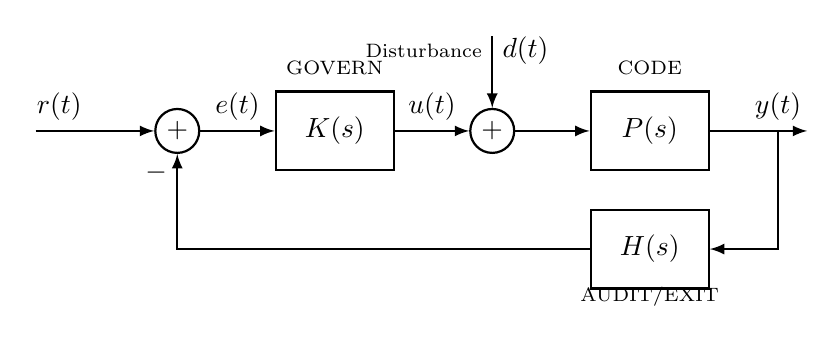
\begin{tikzpicture}[node distance=1.8cm, auto, >=latex, thick]
    % Styles
    \tikzstyle{block} = [draw, rectangle, minimum height=1cm, minimum width=1.5cm]
    \tikzstyle{sum} = [draw, circle, inner sep=2pt]
    \tikzstyle{input} = [coordinate]
    \tikzstyle{output} = [coordinate]

    % Nodes
    \node [input] (rinput) {};
    \node [sum, right of=rinput] (sum1) {$+$};
    \node [block, right of=sum1, node distance=2cm] (K) {$K(s)$};
    \node [sum, right of=K, node distance=2cm] (sum2) {$+$};
    \node [block, right of=sum2, node distance=2cm] (P) {$P(s)$};
    \node [output, right of=P, node distance=2cm] (output) {};
    \node [block, below of=P, node distance=1.5cm] (H) {$H(s)$};
    \node [input, above of=sum2, node distance=1.2cm] (disturbance) {};

    % Labels
    \node [above of=K, node distance=0.8cm] {\scriptsize GOVERN};
    \node [below of=H, node distance=0.6cm] {\scriptsize AUDIT/EXIT};
    \node [above of=P, node distance=0.8cm] {\scriptsize CODE};

    % Connections
    \draw [->] (rinput) -- node[pos=0.2] {$r(t)$} (sum1);
    \draw [->] (sum1) -- node {$e(t)$} (K);
    \draw [->] (K) -- node {$u(t)$} (sum2);
    \draw [->] (sum2) -- (P);
    \draw [->] (P) -- node [name=y, pos=0.7] {$y(t)$} (output);
    \draw [->] (y) |- (H);
    \draw [->] (H) -| node[pos=0.9, left] {$-$} (sum1);
    \draw [->] (disturbance) -- node[pos=0.2, right] {$d(t)$} node[pos=0.2, left] {\scriptsize Disturbance} (sum2);
\end{tikzpicture}
\caption{\textbf{Control-theoretic model of corrigible infrastructure.} $K(s)$: governance controller. $H(s)$: sensor/audit function. $P(s)$: plant (infrastructure). $d(t)$: environmental disturbance.}
\label{fig:control-model}
\end{figure}

The closed-loop transfer function from reference to output is:
\begin{equation}
\frac{Y(s)}{R(s)} = \frac{K(s)P(s)}{1 + K(s)P(s)H(s)}
\end{equation}

The transfer function from disturbance to output is:
\begin{equation}
\frac{Y(s)}{D(s)} = \frac{P(s)}{1 + K(s)P(s)H(s)}
\end{equation}

Corrigibility requires that each component exists and is non-degenerate:
\begin{itemize}
    \item EXIT $\Rightarrow$ $e(t) \neq 0$ observable (error signal exists)
    \item AUDIT $\Rightarrow$ $H(s) \neq 0$ (sensor functional)
    \item GOVERN $\Rightarrow$ $K(s) \neq 0$ (actuator functional)
    \item CODE $\Rightarrow$ $P(s)$ is intelligible
    \item FORK $\Rightarrow$ $P, K, H$ replaceable if convergence fails
\end{itemize}

\begin{figure}[htbp]
\centering
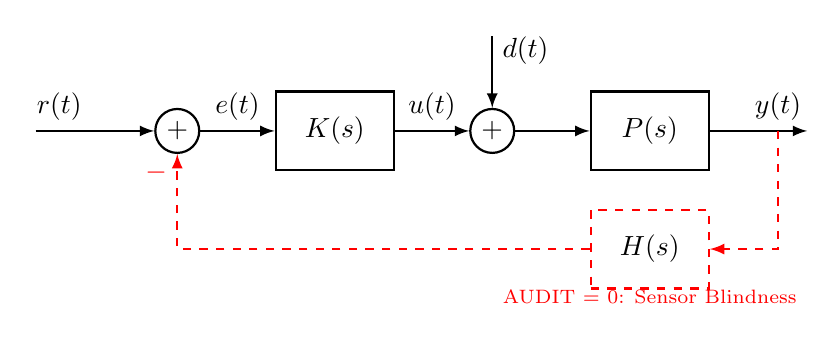
\begin{tikzpicture}[node distance=1.8cm, auto, >=latex, thick]
    \tikzstyle{block} = [draw, rectangle, minimum height=1cm, minimum width=1.5cm]
    \tikzstyle{sum} = [draw, circle, inner sep=2pt]
    \tikzstyle{input} = [coordinate]
    \tikzstyle{output} = [coordinate]

    \node [input] (rinput) {};
    \node [sum, right of=rinput] (sum1) {$+$};
    \node [block, right of=sum1, node distance=2cm] (K) {$K(s)$};
    \node [sum, right of=K, node distance=2cm] (sum2) {$+$};
    \node [block, right of=sum2, node distance=2cm] (P) {$P(s)$};
    \node [output, right of=P, node distance=2cm] (output) {};
    \node [block, below of=P, node distance=1.5cm, draw=red, dashed] (H) {$H(s)$};
    \node [input, above of=sum2, node distance=1.2cm] (disturbance) {};

    \node [below of=H, node distance=0.6cm, red] {\scriptsize AUDIT = 0: Sensor Blindness};

    \draw [->] (rinput) -- node[pos=0.2] {$r(t)$} (sum1);
    \draw [->] (sum1) -- node {$e(t)$} (K);
    \draw [->] (K) -- node {$u(t)$} (sum2);
    \draw [->] (sum2) -- (P);
    \draw [->] (P) -- node [name=y, pos=0.7] {$y(t)$} (output);
    \draw [->, dashed, red] (y) |- (H);
    \draw [->, dashed, red] (H) -| node[pos=0.9, left] {$-$} (sum1);
    \draw [->] (disturbance) -- node[pos=0.2, right] {$d(t)$} (sum2);
\end{tikzpicture}
\caption{\textbf{Open-loop failure mode.} When AUDIT fails ($H = 0$), the feedback path is severed. Equivalent failure occurs if GOVERN ($K = 0$) or EXIT ($e(t) \equiv 0$) is removed.}
\label{fig:open-loop}
\end{figure}

\subsection{The Strict Correction Velocity Inequality}

For the system to remain stable not just asymptotically but locally (preventing irreversible harm), the correction rate must dominate the error rate. We formalize this with a friction coefficient.

\begin{condition}[Strict Dynamic Stability]
Let $\epsilon > 0$ represent the ``friction cost'' of correction (e.g., litigation time, protest cost). A system is stable iff:
\begin{equation}
\left| \frac{d}{dt} C(t) \right| \ge \left| \frac{d}{dt} E(t) \right| + \epsilon
\end{equation}
\end{condition}

\textbf{Implication:} Post-hoc remedies (Courts/Ombudsmen) have a linear or constant rate of operation ($\frac{dC}{dt} = k$). Digital errors propagate at exponential or high-frequency rates ($\frac{dE}{dt} \propto e^{t}$). Since there is no $t$ for which a linear function dominates an exponential one, relying on external courts guarantees eventual system collapse. The correction logic must be intrinsic to the loop.

\begin{figure}[htbp]
\centering
\begin{tikzpicture}[scale=0.9]
    \begin{axis}[
        xlabel={Time},
        ylabel={Magnitude},
        xmin=0, xmax=5,
        ymin=0, ymax=10,
        legend pos=north west,
        axis lines=left,
        domain=0:5,
        samples=100,
        width=10cm,
        height=6cm
    ]
    \addplot[blue, thick, name path=E] {1.5*exp(0.5*x)};
    \addlegendentry{$E(t)$ Error accumulation}
    \addplot[green!60!black, thick, name path=C] {1 + 0.8*x};
    \addlegendentry{$C(t)$ Correction capacity}
    \addplot[red!30, opacity=0.5] fill between[of=E and C, soft clip={domain=1.5:5}];
    \node at (axis cs:3.5,6) {\scriptsize Instability};
    \end{axis}
\end{tikzpicture}
\caption{\textbf{Correction velocity mismatch.} Error $E(t)$ accumulates faster than correction $C(t)$ in bureaucratic systems. The shaded region represents accumulated unresolved harm.}
\label{fig:velocity-mismatch}
\end{figure}

\subsection{Mapping to the Five Tests}

\begin{table}[htbp]
\centering
\caption{Mapping corrigibility tests to control-theoretic components}
\label{tab:control-mapping}
\begin{tabular}{lll}
\hline
\textbf{Test} & \textbf{Control Component} & \textbf{Failure Mode} \\
\hline
EXIT & Error Signal & Reference collapse \\
CODE & Signal Integrity & Noise indistinguishable from intent \\
AUDIT & Sensor & Blind control \\
GOVERN & Actuator & No corrective force \\
FORK & Variety Expansion & Monolithic collapse \\
\hline
\end{tabular}
\end{table}

\subsection{Agentic Interoperability Requirements}

For an autonomous agent $\mathcal{A}$ to operate reliably within infrastructure $\mathcal{I}$, the following predicates must be strictly True:

\begin{enumerate}
    \item \textbf{Reversibility:} $\forall$ state $s_t \in \mathcal{S}$, $\exists$ transition $s_{t+1}$ (via \texttt{EXIT}) such that $\text{Cost}(s_{t+1}) < \infty$. (No deadlocks).
    \item \textbf{Decidability:} $\forall$ input $x$, $\text{Compute}(x) \to \{0,1\}$ is inspectable via \textbf{CODE}. (No hidden constraints).
\end{enumerate}

Failure of these predicates renders $\mathcal{I}$ a ``Hazmat Environment'' for automated agents, effectively blocking the agentic economy.

\begin{figure}[htbp]
\centering
\begin{tikzpicture}[node distance=2cm, auto, >=latex, thick]
    \tikzstyle{state} = [draw, ellipse, minimum width=1.5cm, minimum height=1cm]
    \tikzstyle{blocked} = [draw, ellipse, minimum width=1.5cm, minimum height=1cm, fill=red!20]

    \node [state] (idle) {Idle};
    \node [state, right of=idle, node distance=3cm] (call) {Call API};
    \node [state, right of=call, node distance=3cm] (success) {Success};
    \node [blocked, below of=call, node distance=2cm] (blocked) {Blocked};
    \node [state, below of=success, node distance=2cm] (error) {Error};

    \draw [->] (idle) -- node {\scriptsize request} (call);
    \draw [->] (call) -- node {\scriptsize 2xx} (success);
    \draw [->] (success) -- node {\scriptsize done} ++(1.5,0);
    \draw [->] (call) -- node[left] {\scriptsize blocked} (blocked);
    \draw [->] (call) to[bend left=30] node[above] {\scriptsize retry} (call);
    \draw [->] (call) -- node {\scriptsize timeout} (error);
    \draw [->] (blocked) -- node[below] {\scriptsize (No Exit)} ++(-2,0);
\end{tikzpicture}
\caption{\textbf{Agentic automaton.} Without EXIT and observable error codes, agent loops indefinitely, times out, or escalates incorrectly.}
\label{fig:agentic-automaton}
\end{figure}

\subsection{Operational Proxies and Thresholds}

\begin{table}[htbp]
\centering
\caption{Operational proxies for the five tests. Thresholds are illustrative.}
\label{tab:operational-proxies}
\begin{tabular}{lll}
\hline
\textbf{Test} & \textbf{Proxy Metric} & \textbf{Illustrative Threshold} \\
\hline
EXIT & Penalty ratio $p$ & $p \leq 1.2$ \\
CODE & Visibility fraction $v$ & $v \geq 0.9$ \\
AUDIT & Mean time to detect (MTTD) & MTTD $\leq$ 24 hours \\
GOVERN & Bindingness + throughput $\tau$ & binding = true, $\tau \geq 1$ per 10k users/day \\
FORK & Resource feasibility ratio $r$ & $r \leq 10^{-3}$ \\
\hline
\end{tabular}
\end{table}

\textbf{Interpretation:}
\begin{itemize}
    \item Penalty ratio $p$ = cost(non-digital alternative) / cost(digital).
    \item Visibility $v$ = public LOC / total LOC on critical execution path.
    \item Resource ratio $r$ = estimated FLOP to retrain / aggregate community compute capacity.
\end{itemize}

\subsection{Network Adoption Model for Fork Feasibility}

Model adoption fraction $\alpha(t)$. A community-spawned fork succeeds if $\alpha$ crosses critical mass $\alpha^*$. Logistic adoption with social influence:
\begin{equation}
\dot{\alpha} = \beta \alpha(1 - \alpha) + s(t)
\end{equation}
where $s(t)$ is exogenous seeding. Fork feasibility requires parameters such that $\exists t$ with $\alpha(t) \geq \alpha^*$. Practical condition:
\begin{equation}
s_{\min} \geq \alpha^* - \alpha_0
\end{equation}
or subsidies that accelerate adoption rate $\beta$.

\begin{figure}[htbp]
\centering
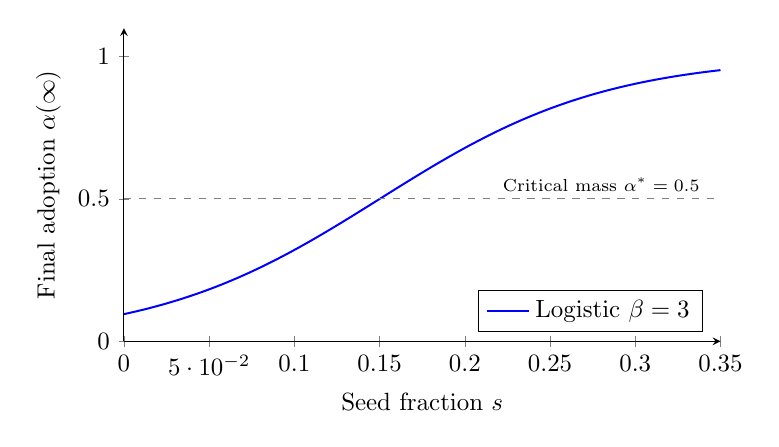
\begin{tikzpicture}[scale=0.9]
    \begin{axis}[
        xlabel={Seed fraction $s$},
        ylabel={Final adoption $\alpha(\infty)$},
        xmin=0, xmax=0.35,
        ymin=0, ymax=1.1,
        legend pos=south east,
        axis lines=left,
        width=10cm,
        height=6cm
    ]
    \addplot[blue, thick, domain=0:0.35, samples=100] {1/(1+exp(-15*(x-0.15)))};
    \addlegendentry{Logistic $\beta = 3$}
    \draw[dashed, gray] (axis cs:0,0.5) -- (axis cs:0.35,0.5);
    \node at (axis cs:0.28,0.55) {\scriptsize Critical mass $\alpha^* = 0.5$};
    \end{axis}
\end{tikzpicture}
\caption{\textbf{Fork feasibility curve.} Below critical seeding, adoption does not reach critical mass. Parameters illustrative.}
\label{fig:fork-feasibility}
\end{figure}

\subsection{Summary of Formal Extensions}

\begin{enumerate}
    \item Linearized result ties removal of $H$, $K$, or EXIT to vanishing loop gain $L(s)$, exposing unstable process modes.
    \item Integrator example supplies simple, indisputable divergence demonstration.
    \item Correction velocity formalized via measurable $C(t)$ and $E(t)$.
    \item Network model clarifies why legal forkability may fail in practice and yields policy levers (seeding, subsidies).
    \item Agent automaton demonstrates need for explicit machine-facing EXIT/CODE/AUDIT primitives.
\end{enumerate}